
\begin{frame}{The basic problem}

%\adjincludegraphics[width=0.9\textwidth,trim={0 {.5\height} 0 0 }, clip]{static_figures/survey_and_voting.jpg}

We have a survey population, for whom we observe:
%
\begin{itemize}
 \item Covariates $\x$ (e.g.~race, gender, zip code, age, education level)
 \item Responses $\y$ (e.g.~A binary response to ``do you support policy such--and--such'')
\end{itemize}
%

We want the average response in a target population,
in which we observe only covariates.



\begin{minipage}{0.45\textwidth}
    \centering
    \only<1>{
    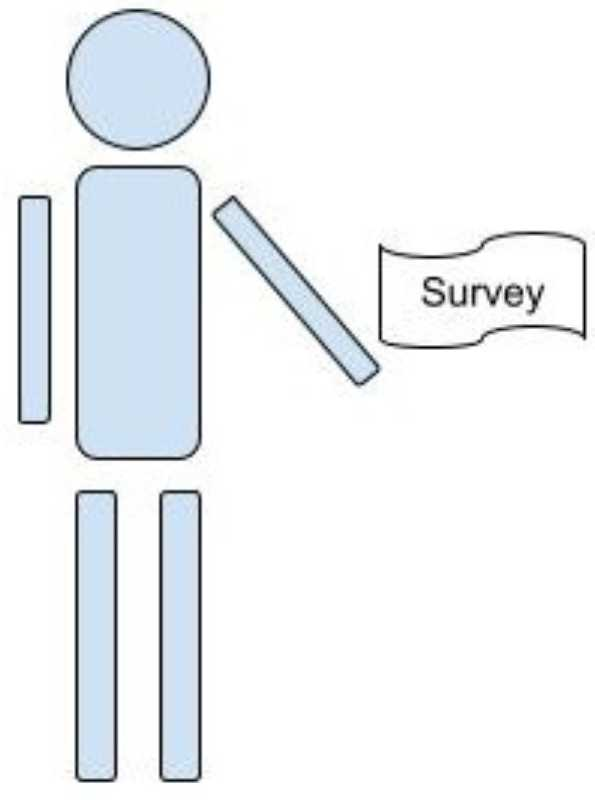
\includegraphics[width=0.5\textwidth]{static_figures/survey_man.jpg}
    }
    \only<2->{
    
\includegraphics[width=0.5\textwidth]{static_figures/survey_crazy_man.jpg}
    }
\end{minipage}
\begin{minipage}{0.45\textwidth}
    \centering
    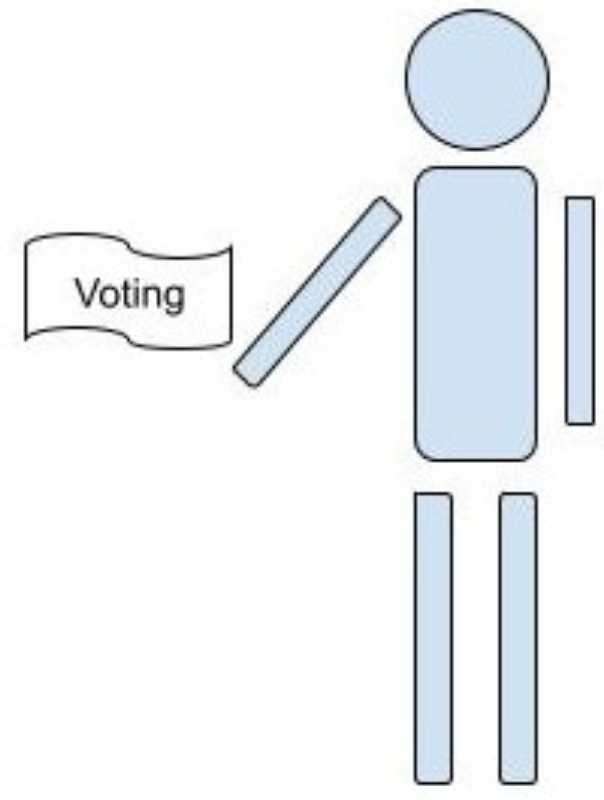
\includegraphics[width=0.5\textwidth]{static_figures/voting_man.jpg}
\end{minipage}

\begin{minipage}{0.45\textwidth}
    \centering
    Observe $(\x_s, y_s)$ for $s = 1, \ldots, \nsur$\\
\end{minipage}
\begin{minipage}{0.45\textwidth}
    \centering
    Observe $\x_p$ for $p = 1, \ldots, \ntar$\\
\end{minipage}

\onslide<2->{
\textbf{The problem is that the populations are very different.}
}

\onslide<3->{
    Our survey results may be biased.

    How can we use the covariates
    to say something about the target responses?
}
%
\end{frame}


\begin{frame}{Two approaches}

We want $\mu := \meantar \y_p$, but don't observe $\y_p$ in the target population.

\begin{itemize}
    \item Assume $p(y | x)$ is the same in both populations,
    \item But the distribution of $x$ may be different in the survey and target.
\end{itemize}
%

\begin{minipage}{0.45\textwidth}
    \centering
    \textbf{Calibration weighting}

    Use

    $\muhat_{\cal} := \meansur w_s y_s$

    For some weights $w_s$ on the survey data.
\end{minipage}
\hfill\vrule\hfill
\begin{minipage}{0.45\textwidth}
    \centering
    \textbf{Model--based}
\end{minipage}

\end{frame}